\section{Holiday and Sick Leave Detection}

Figure~\ref{fig:missing-time} shows the analysis of an employee for their employer's repositories.
The y-axis represents the additions and deletions of commits, the x-axis represents the week of the respective year.
For better verification and evaluation of the results, a scatter plot with the additions and deletions of each commit has been added on top of individual miss-out graphs.

\begin{figure}[h]
    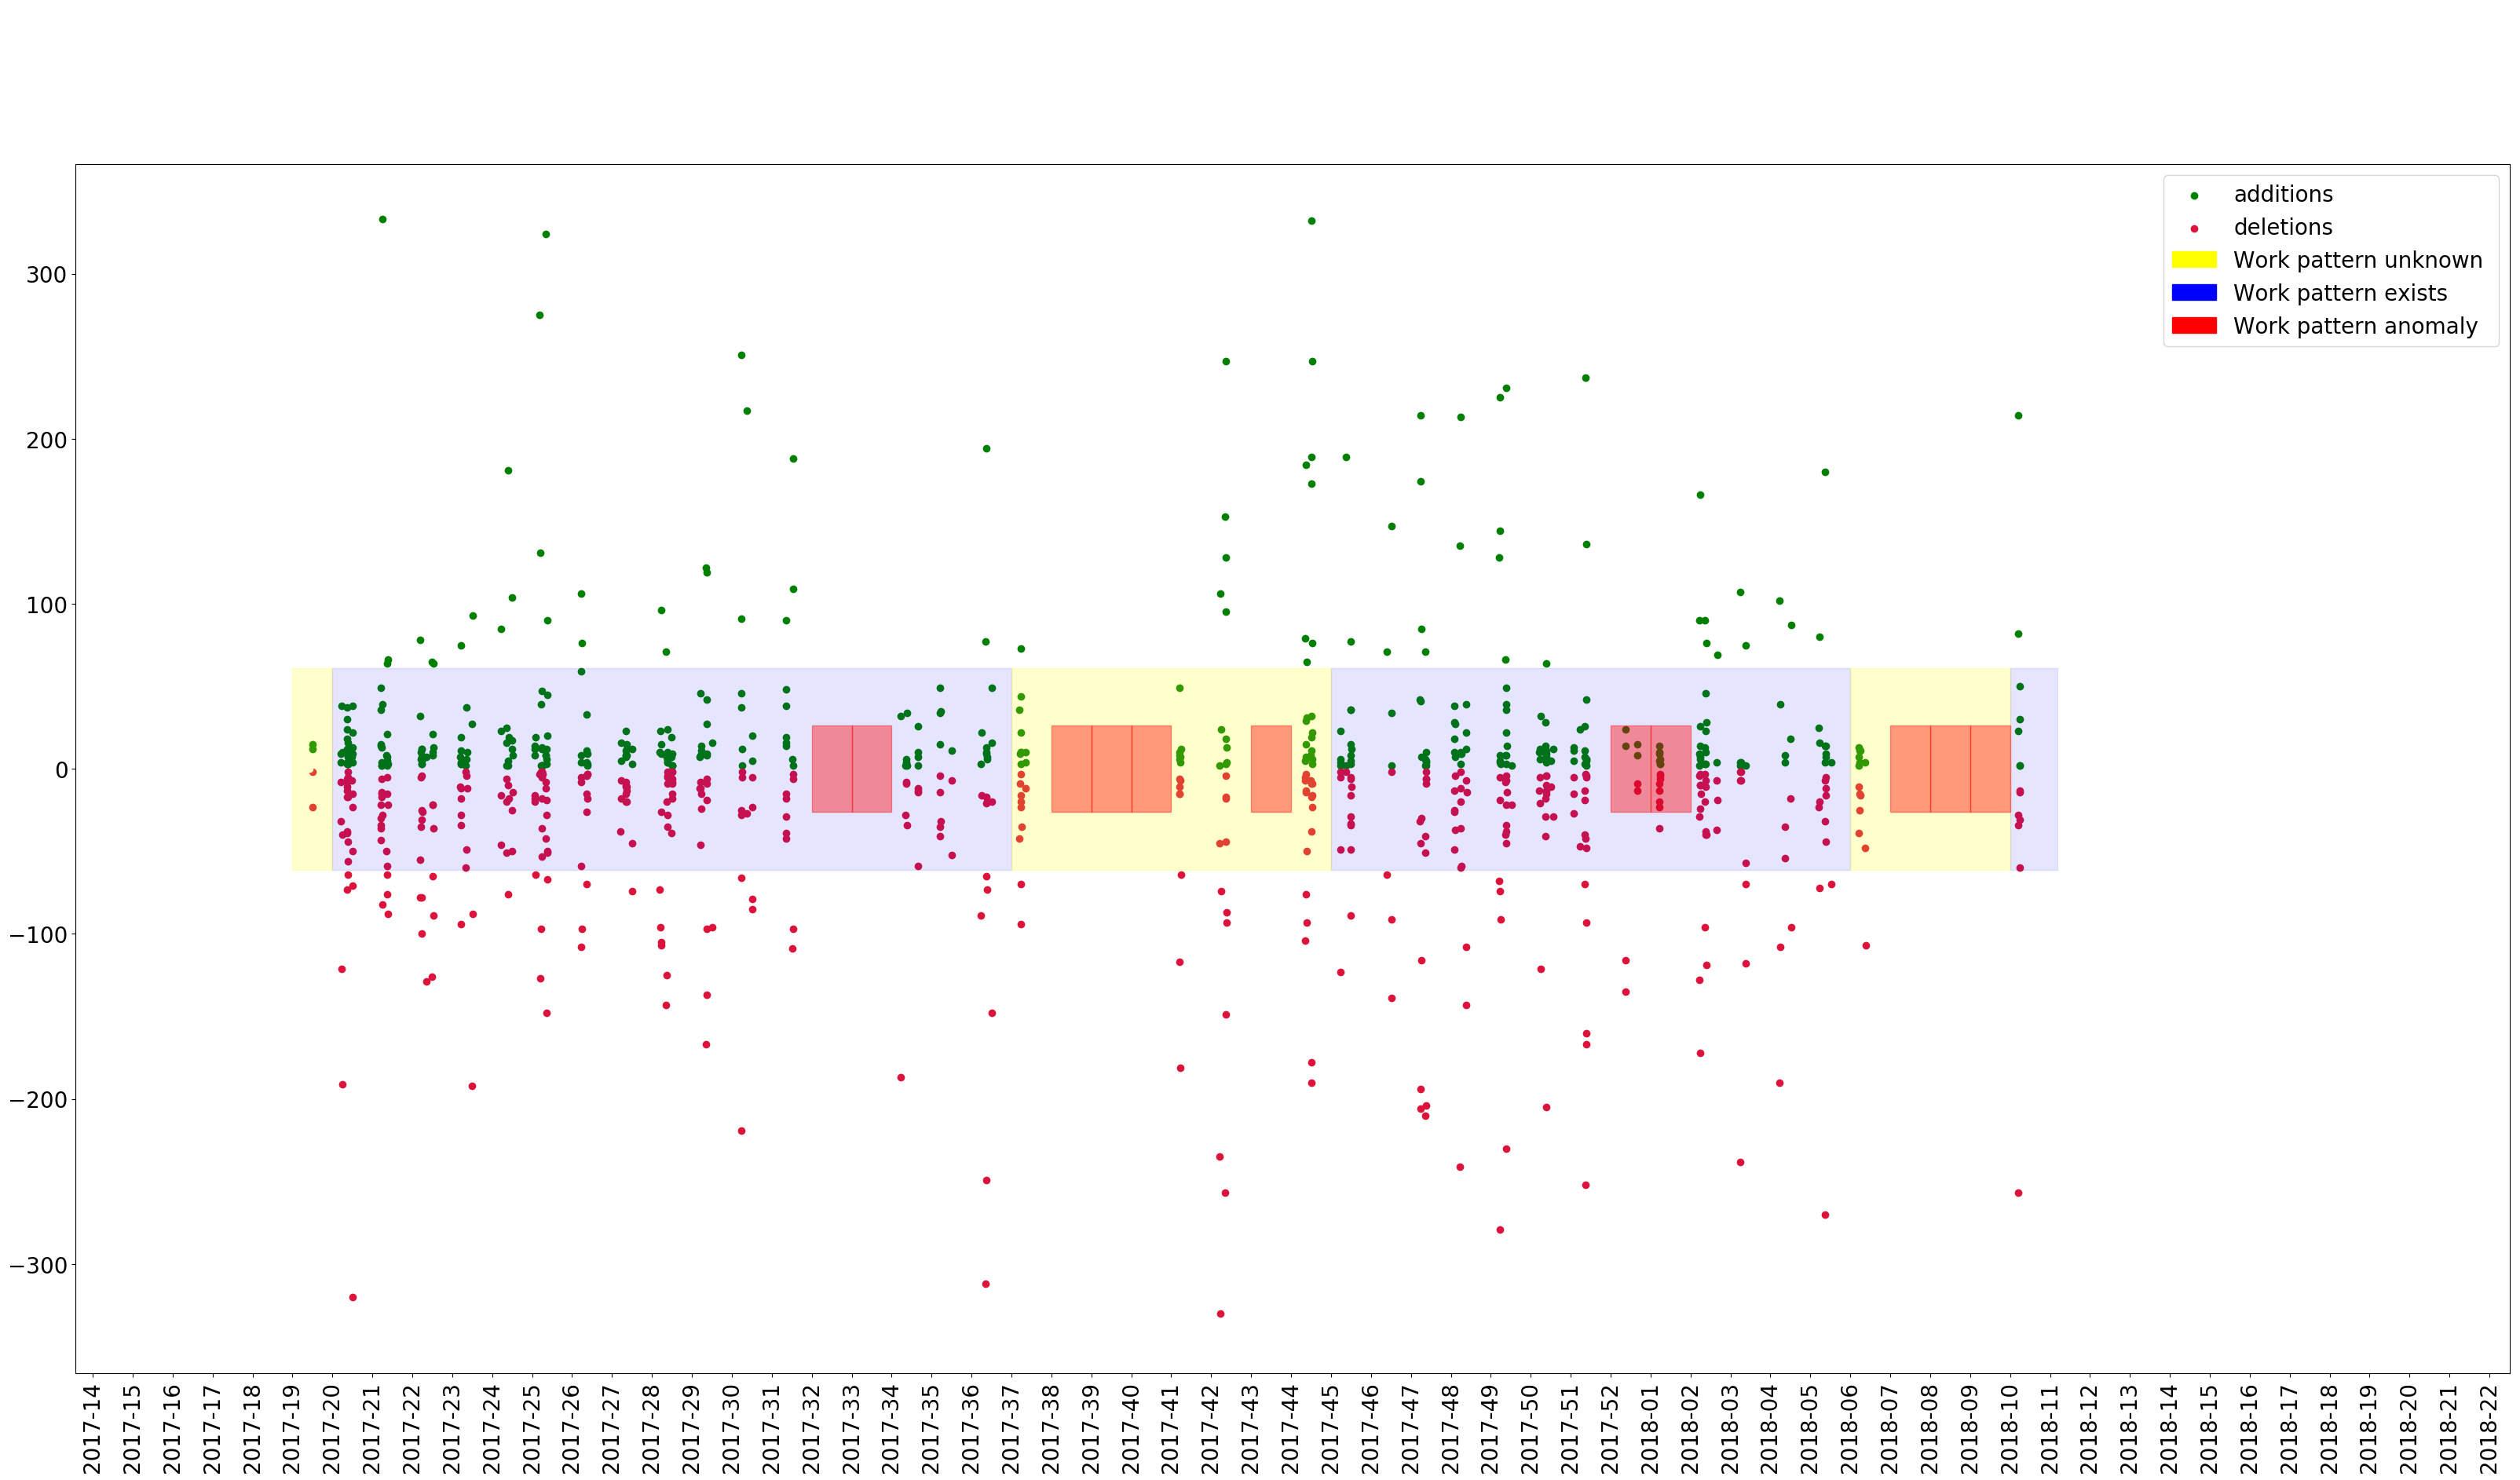
\includegraphics[scale=0.19]{./graphs/analysis/work-time-analysis}
    \centering
    \caption{
        The work time analysis of an employee.
        Blue sections are time spans in which the target has a consistent reoccurring week work pattern.
        Yellow sections show irregularities in their week work pattern.
        Red blocks are miss-out anomalies detected by the algorithm, which indicate holiday or sick leave.
    }\label{fig:missing-time}
\end{figure}

The evaluation of this algorithm turned out to be quite difficult, as there is no publicly available information about sick leave or holiday.
For the purpose of this thesis, I was allowed to use anonymous statistics of a company with a test group of five developing employees.

After scanning and analyzing the company's repositories, a survey has been conducted, for which each employee had to look at their visualized miss-out graph and check whether there are any wrong or missing detections.

The algorithm successfully managed to find all sick leave and holiday-related miss-outs in all cases.
However, there were three false positive cases.
Firstly a developer did work related research and did thereby not commit as regularly as usual, which was then detected as a miss-out.
Secondly, a developer contributed to repositories, which are not owned by the employee.
As a result, two weeks were marked as miss-out.
Thirdly there were two developers, that contributed to a branch, but their work has not been merged into the master branch yet, hence the commits were not being scanned yet.
This particular problem can be solved by not only scanning the master branch but also all other branches, however, this adds a lot of complexity to the continuous mining process and has thereby not been implemented yet.
Anyway, this problem only seems to occur in the latest weeks.

A not intended side effect of detecting prototypes is that the algorithm not only detected anomalies, such as sick leave or holiday, but also found inconsistencies in the work routine.
For instance between week 37 to 45 in Figure~\ref{fig:missing-time}, a developer was forced to reduce their working hours due to legal questions and continuously shifted hours and working days for several weeks.
It is hard to interpret those inconsistencies without more contextual information, but nevertheless, it provides the fact that something happened during this time.

The conducted survey also included a question about the precision of these inconsistencies.
In the case of three developers, the inconsistencies perfectly matched real-world occurrences in their work behavior.
In the two remaining cases, there were a few inconsistencies the developers could not explain, even though there definitely were inconsistencies in their commit pattern.
But those inconsistencies could be explained by the fact that those developers were working on flexible work time.

\begin{figure}[h]
    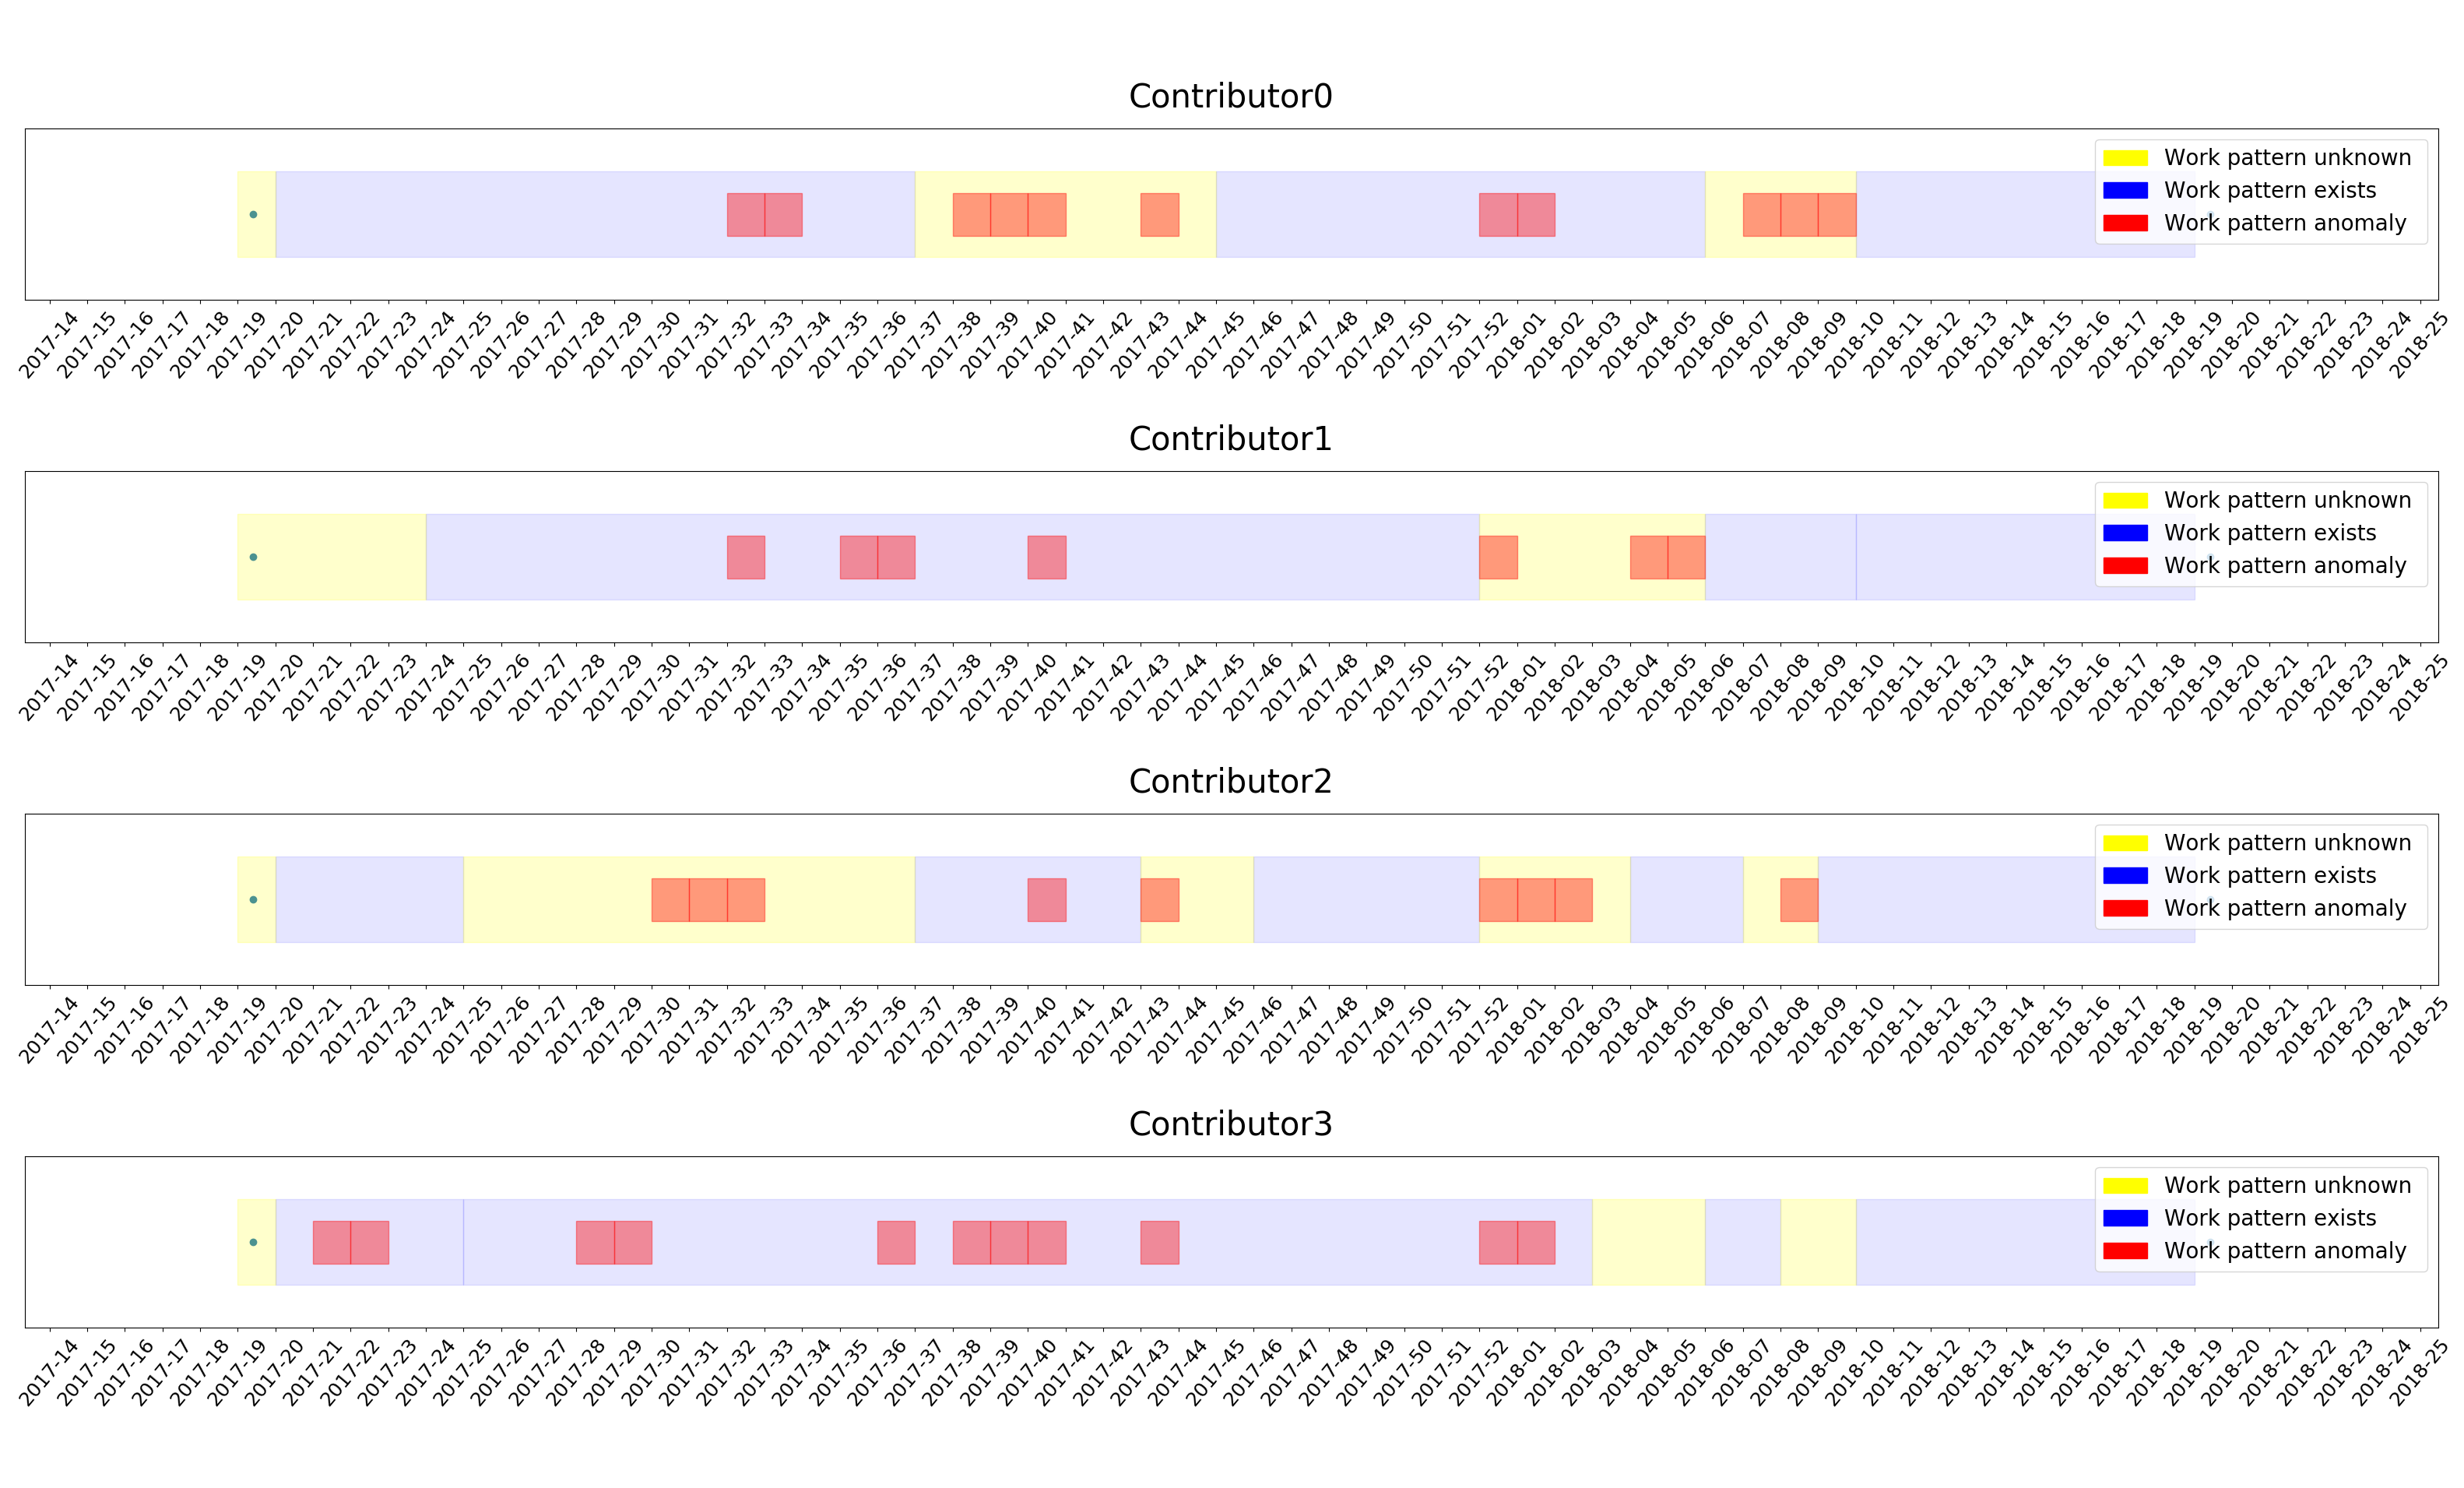
\includegraphics[scale=0.19]{./graphs/analysis/work-time-analysis-comparison}
    \centering
    \caption{The miss-out analysis graphs of the four employees from the survey.}\label{fig:miss-out-comparison}
\end{figure}

In Figure~\ref{fig:miss-out-comparison} the comparison between multiple employees can be seen.
\emph{Contributor0} and \emph{Contributor2} are working on flexible work time, which reflects in the inconsistencies in the work patterns (yellow sections in Figure~\ref{fig:miss-out-comparison}) of those contributors.
The other two contributors have very consistent working hours patterns, as can be seen by the long-lasting blue sections.
